\documentclass{article}
\usepackage{tikz}
\usetikzlibrary{arrows,shapes}
\begin{document}
\pagestyle{empty}

\begin{tikzpicture}[scale=1.5]
    % Draw axes
    \draw [<->,thick] (0,5) node (yaxis) [above] {$x_2$}
        |- (5,0) node (xaxis) [right] {$x_1$};
    % Draw two intersecting lines
    \draw (0,0) coordinate (a_1) -- (1.6,2) coordinate (a_2);
    \draw (1.6,2) coordinate (b_1) -- (1.6,4.75) coordinate (b_2);
    \draw[dashed] (0,4.88) -- (2.7111,0);
    \node at (3.4,0.4) {$s_2(\bar W(t))=K_2$};

    \coordinate (c) at (intersection of a_1--a_2 and b_1--b_2);
    % Draw lines indicating intersection with y and x axis. Here we use
    % the perpendicular coordinate system
    \draw[dashed] (yaxis |- c) node[left] {$K_2$}
        -| (xaxis -| c) node[below] {$\frac{\mu_2K_2}{\mu_1}$};
    \draw[dashed] (2.2, 0.05) -- (2.2,0) node[below] {$K_1$};
    % Draw a dot to indicate intersection point
    
    \coordinate (a) at (2.4,0.8);
    \fill[red] (a) circle (1pt);
    \draw[blue] (a) -- (1.6,0.8);

    \coordinate (b) at (1.94,0.9);
    \fill[red] (b) circle (1pt);
    \draw[blue] (b) -- (1.44,1.8);

\end{tikzpicture}

\begin{figure}[h]\label{fig:N-model-rework}
  \centering
  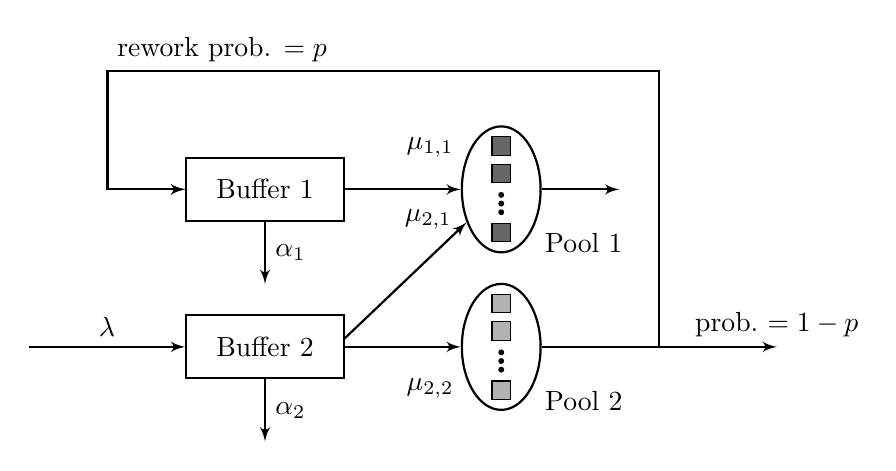
\begin{tikzpicture}[auto, >=latex']
    \everymath{\displaystyle}
    \tikzstyle{every picture}+=[remember picture]

    \tikzstyle{coor-format} = [coordinate]
    \tikzstyle{b-format} = [draw=black, thick,
                            minimum height=0.8cm, minimum width=2cm]
    \tikzstyle{s1-format} = [rectangle, draw=black, fill=black!60]
    \tikzstyle{s2-format} = [rectangle, draw=black, fill=black!30]
    \tikzstyle{p-format} = [ellipse, draw=black, thick,
                            minimum height=1.6cm, minimum width=1cm]

    \node [coor-format] (In1) {};
    \node [b-format, right of=In1, node distance=2cm] (Buf1) {Buffer 1};
    \draw [draw,->, thick] (In1) -- (Buf1);

    \node [coor-format, below of=Buf1, node distance=1.2cm] (Abd1) {};
    \draw [draw,->, thick] (Buf1) -- node {$\alpha_1$} (Abd1);

    \node [p-format, right of=Buf1, node distance=3cm, label=-45:Pool 1,
           label=150:{$\mu_{1,1}$}, label=-165:{$\mu_{2,1}$}] (Pool1) {};
    \draw [draw,->, thick] (Buf1) -- (Pool1);

    \node [coor-format, right of=Pool1, node distance=1.5cm] (Out1) {};
    \draw [draw,->, thick] (Pool1) -- (Out1);

    \node [coor-format,below of = In1, node distance = 2cm] (In2) {};
    \node [b-format, right of=In2, node distance=2cm] (Buf2) {Buffer 2};
    \draw [draw,->, thick] (In2)+(-1cm,0) --node {$\lambda$} (Buf2);

    \node [p-format, right of=Buf2, node distance=3cm,
           label=-45:Pool 2,label=-150:$\mu_{2,2}$] (Pool2) {};
    \draw [draw,->, thick] (Buf2) -- (Pool2);
    \draw [draw,->, thick] (Buf2.east)+(-0.01cm,0.1cm) -- (Pool1);

    \node [coor-format, below of=Buf2, node distance=1.2cm] (Abd2) {};
    \draw [draw,->, thick] (Buf2) -- node {$\alpha_2$} (Abd2);

    \node [coor-format, right of=Pool2, node distance=3.5cm,
    label=90:{prob.\ $=1-p$}] (Out2) {};
    \draw [draw,->, thick] (Pool2) -- (Out2);

    \node [coor-format, above of = In1,
           node distance=1.5cm, label=45:rework prob. {$=p$}](upper-left){};
    \path [draw, -, thick] (Out2)+(-1.5cm,0) |- (upper-left);

    \draw [draw, ->, thick] (upper-left)+(0,0.014cm) |- (Buf1);

    \node at (5cm,0.55cm) [s1-format]{};
    \node at (5cm,0.2cm) [s1-format]{};
    \draw [draw=black, fill=black]
           (5cm,-0.07cm) circle (0.03cm);
    \draw [draw=black, fill=black]
           (5cm,-0.18cm) circle (0.03cm);
    \draw [draw=black, fill=black]
           (5cm,-0.29cm) circle (0.03cm);
    \node at (5cm,-0.55cm) [s1-format]{};

    \node at (5cm,0.55cm-2cm) [s2-format]{};
    \node at (5cm,0.2cm-2cm) [s2-format]{};
    \draw [draw=black, fill=black]
           (5cm,-0.07cm-2cm) circle (0.03cm);
    \draw [draw=black, fill=black]
           (5cm,-0.18cm-2cm) circle (0.03cm);
    \draw [draw=black, fill=black]
           (5cm,-0.29cm-2cm) circle (0.03cm);
    \node at (5cm,-0.55cm-2cm) [s2-format]{};
 \end{tikzpicture}
 \caption{A schematic Model of Outsourcing with rework}
\end{figure}

\end{document}